
\chapter{Artifact Evaluation and Discussion}

In this chapter we will evaluate the artifact from three perspectives:

\begin{enumerate}
    \item Basic web performance metrics;
    \item A systematic collection and analysis of the data produced by the artifact;
    \item Interviews with stakeholders;
\end{enumerate}


\section{Web Performance Metrics}

Using a website speed tester, we can gather useful information about the performance of the artifact, in terms of loading latency. For this test, Pingdom\footnotemark[1] was used.

\footnotetext[1]{https://tools.pingdom.com/}

Three tests were carried out, one for each of the page types:

\begin{enumerate}
    \item The about page;
    \item The artifacts browsing page;
    \item The artifact detail page;
\end{enumerate}

All tests were carried out from Pingdom's North America - USA - Washington DC location.

\subsection{About Page}


\begin{table}[H]
\footnotesize
\centering
\begin{tabular}{|ll|}
\hline
\multicolumn{1}{|l|}{\textbf{Page}} & \textbf{URL}                                                 \\ \hline
\multicolumn{1}{|l|}{About}         & http://arkivo.art/ \\ \hline
\multicolumn{2}{|l|}{\textbf{Full Test}}                                                                    \\ \hline
\multicolumn{2}{|l|}{https://tools.pingdom.com/\#64600c6e88c00000}                                 \\ \hline
\end{tabular}
\caption{Artifacts Browsing - Web Performance Test Details}
\label{table:browsing-test-details}
\end{table}


\begin{figure}[H]
    \centering
    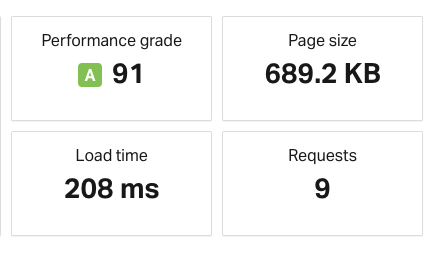
\includegraphics[width=0.5\linewidth]{about-01-general.png}
    \caption[Performance Metric: About Page (Overall)]{Performance Metric: About Page (Overall)}
    \label{fig:about-01-general}
\end{figure}

\begin{figure}[H]
    \centering
    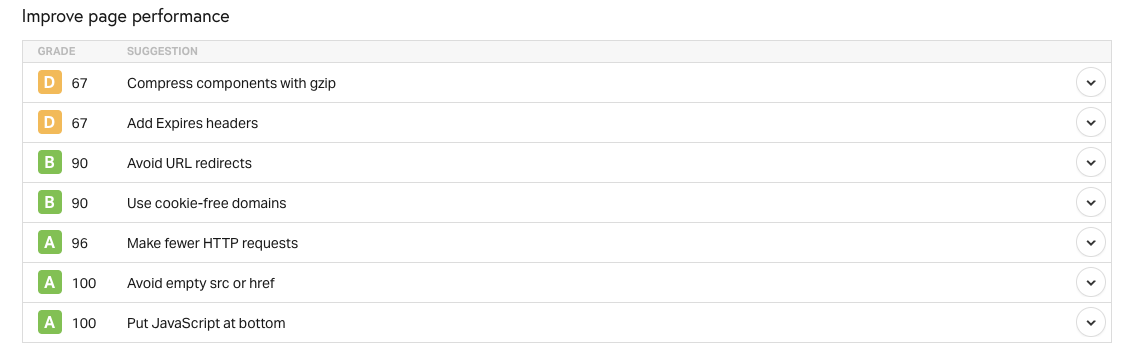
\includegraphics[width=\linewidth]{about-02-perf.png}
    \caption[Performance Metric: About Page (Improvement Areas)]{Performance Metric: About Page (Improvement Areas)}
    \label{fig:about-02-perf.png}
\end{figure}

\begin{figure}[H]
    \centering
    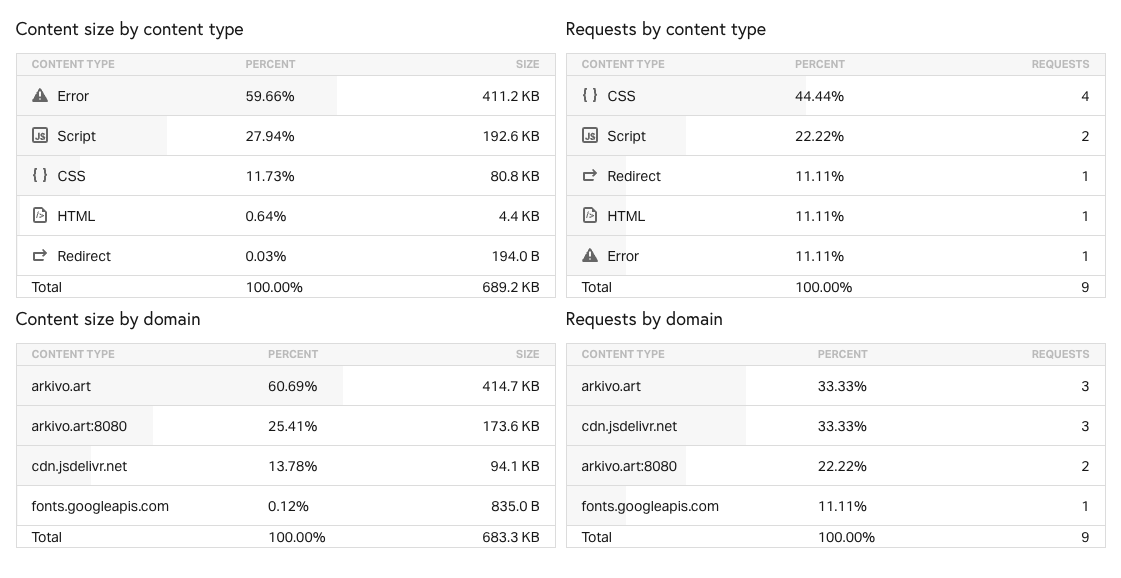
\includegraphics[width=\linewidth]{about-03-stats.png}
    \caption[Performance Metric: About Page (Content Breakdown)]{Performance Metric: About Page (Content Breakdown)}
    \label{fig:about-03-stats.png}
\end{figure}

\begin{figure}[H]
    \centering
    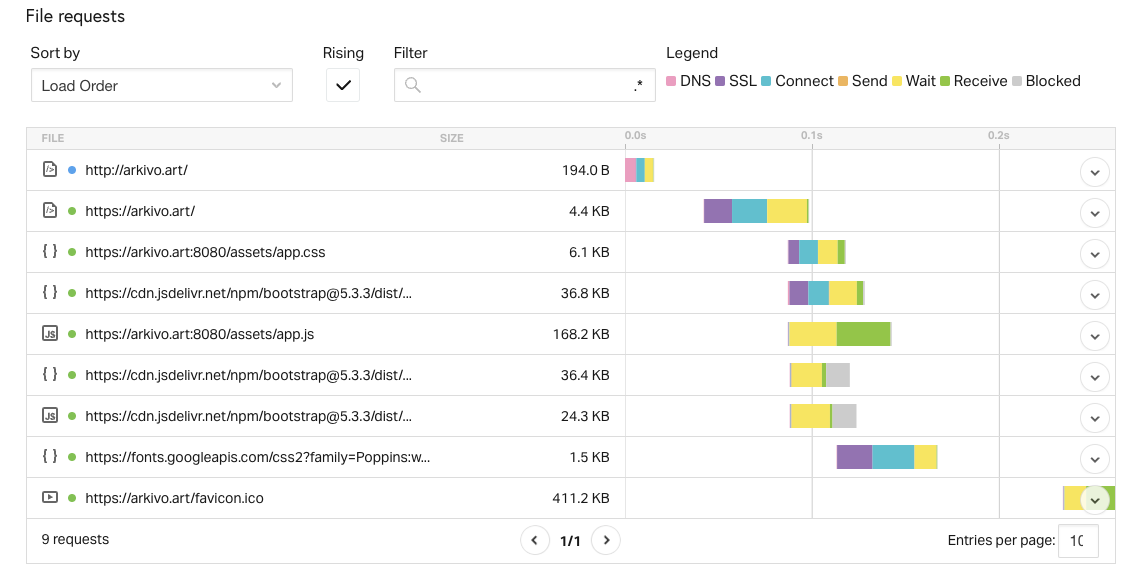
\includegraphics[width=\linewidth]{about-04-latency.png}
    \caption[Performance Metric: About Page (Loading Timeline)]{Performance Metric: About Page (Loading Timeline)}
    \label{fig:about-04-latency.png}
\end{figure}


\subsection{Artifacts Browsing Page}


\begin{table}[H]
\footnotesize
\centering
\begin{tabular}{|ll|}
\hline
\multicolumn{1}{|l|}{\textbf{Page}} & \textbf{URL}                                                 \\ \hline
\multicolumn{1}{|l|}{Artifacts Browsing}         & \multicolumn{1}{r|}{http://arkivo.art/artifacts} \\ \hline
\multicolumn{2}{|l|}{\textbf{Full Test}}                                                                    \\ \hline
\multicolumn{2}{|l|}{https://tools.pingdom.com/\#64600d6d24000000}                                 \\ \hline
\end{tabular}
\caption{Artifacts Browsing - Web Performance Test Details}
\label{table:browsing-test-details}
\end{table}


\begin{figure}[H]
    \centering
    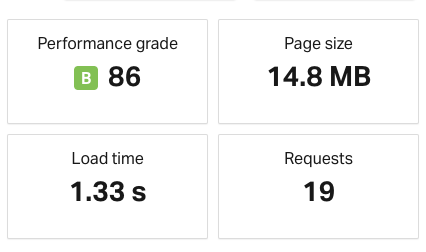
\includegraphics[width=0.5\linewidth]{artifacts-01-general.png}
    \caption[Performance Metric: Artifacts Browsing Page (Overall)]{Performance Metric: Artifacts Browsing Page (Overall)}
    \label{fig:artifacts-01-general}
\end{figure}

\begin{figure}[H]
    \centering
    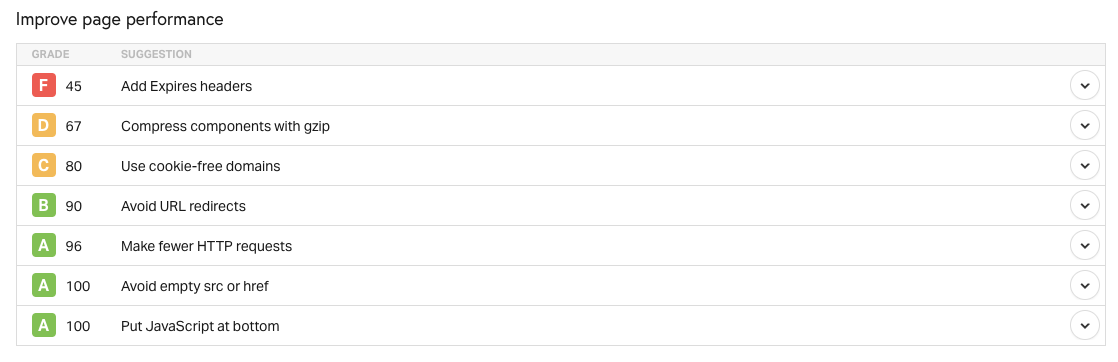
\includegraphics[width=\linewidth]{artifacts-02-perf.png}
    \caption[Performance Metric: Artifacts Browsing Page (Improvement Areas)]{Performance Metric: Artifacts Browsing Page (Improvement Areas)}
    \label{fig:artifacts-02-perf.png}
\end{figure}

\begin{figure}[H]
    \centering
    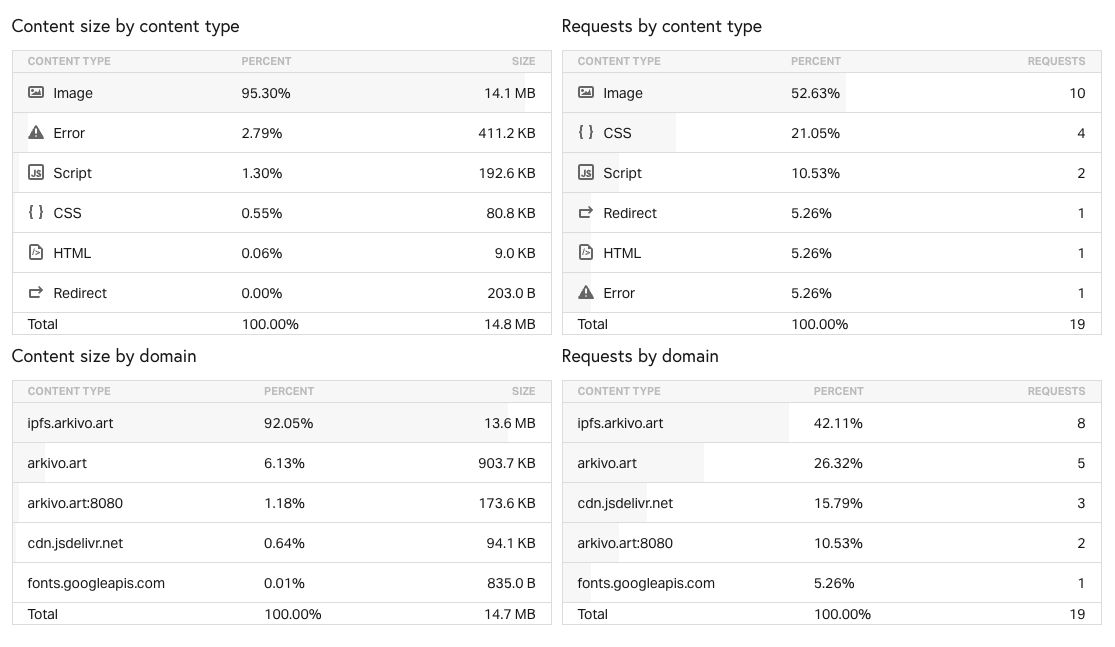
\includegraphics[width=\linewidth]{artifacts-03-stats.png}
    \caption[Performance Metric: Artifacts Browsing Page (Content Breakdown)]{Performance Metric: Artifacts Browsing Page (Content Breakdown)}
    \label{fig:artifacts-03-stats.png}
\end{figure}

\begin{figure}[H]
    \centering
    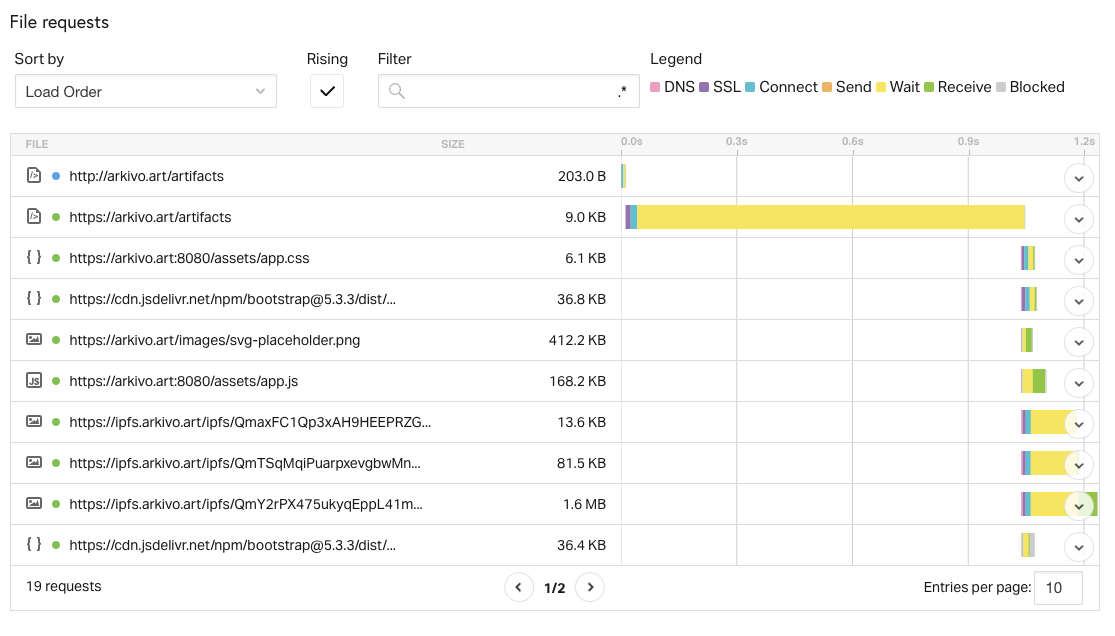
\includegraphics[width=\linewidth]{artifacts-04-latency1.png}
    \caption[Performance Metric: Artifacts Browsing Page (Loading Timeline) 1/2]{Performance Metric: Artifacts Browsing Page (Loading Timeline) 1/2}
    \label{fig:artifacts-04-latency.png}
\end{figure}

\begin{figure}[H]
    \centering
    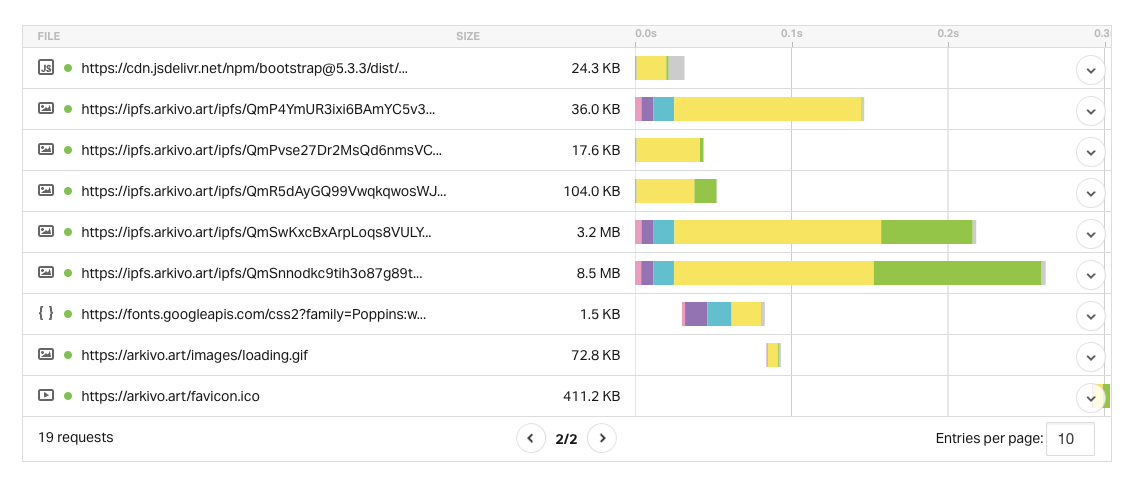
\includegraphics[width=\linewidth]{artifacts-04-latency2.png}
    \caption[Performance Metric: Artifacts Browsing Page (Loading Timeline) 2/2]{Performance Metric: Artifacts Browsing Page (Loading Timeline) 2/2}
    \label{fig:artifacts-04-latency.png}
\end{figure}


\subsection{Artifact Detail Page}

\begin{table}[h]
\footnotesize
\centering
\begin{tabular}{|ll|}
\hline
\multicolumn{1}{|l|}{\textbf{Page}} & \textbf{URL}                                                 \\ \hline
\multicolumn{1}{|l|}{Artifact Detail}         & \multicolumn{1}{r|}{https://arkivo.art/artifacts/HEN/653867} \\ \hline
\multicolumn{2}{|l|}{\textbf{Full Test}}                                                                    \\ \hline
\multicolumn{2}{|l|}{https://tools.pingdom.com/\#64600ebfd5000000}                                 \\ \hline
\end{tabular}
\caption{Artifact Detail - Web Performance Test Details}
\label{table:artifact-test-details}
\end{table}

\begin{figure}[H]
    \centering
    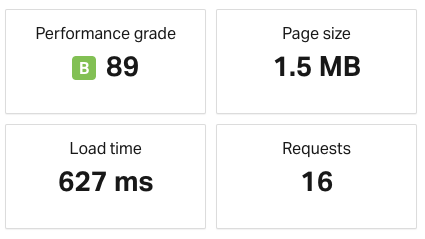
\includegraphics[width=0.5\linewidth]{artifact-01-general.png}
    \caption[Performance Metric: Artifact Detail Page (Overall)]{Performance Metric: Artifact Detail Page (Overall)}
    \label{fig:artifact-01-general}
\end{figure}

\begin{figure}[H]
    \centering
    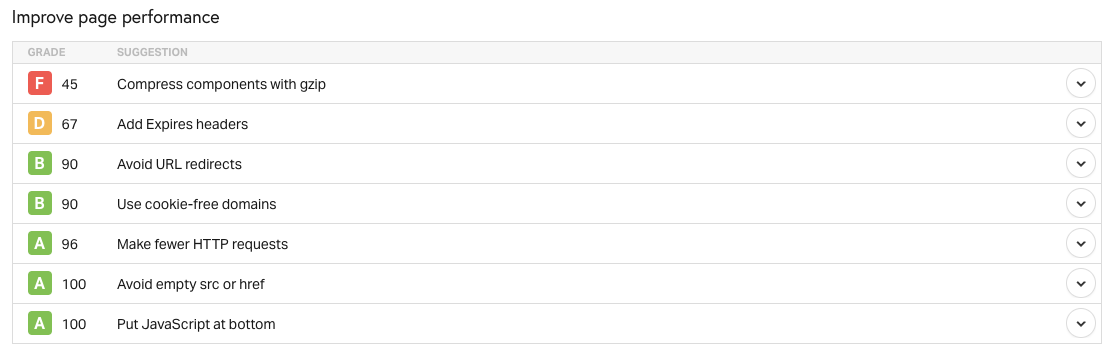
\includegraphics[width=\linewidth]{artifact-02-perf.png}
    \caption[Performance Metric: Artifact Detail Page (Improvement Areas)]{Performance Metric: Artifact Detail Page (Improvement Areas)}
    \label{fig:artifact-02-perf.png}
\end{figure}

\begin{figure}[H]
    \centering
    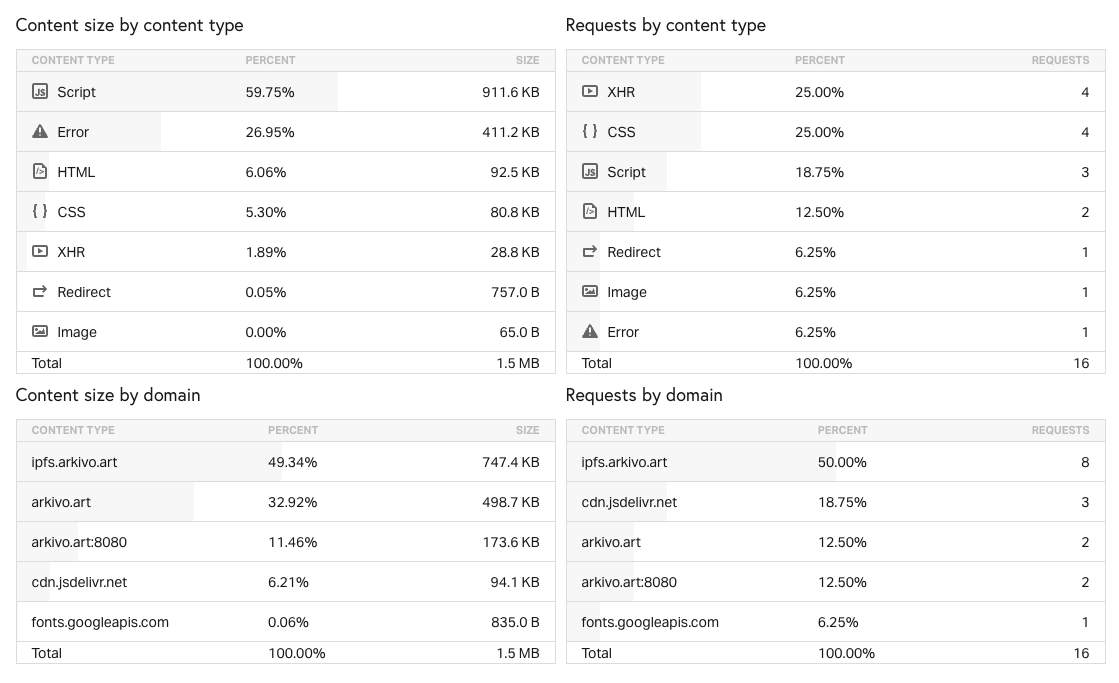
\includegraphics[width=\linewidth]{artifact-03-stats.png}
    \caption[Performance Metric: Artifact Detail Page (Content Breakdown)]{Performance Metric: Artifact Detail Page (Content Breakdown)}
    \label{fig:artifact-03-stats.png}
\end{figure}

\begin{figure}[H]
    \centering
    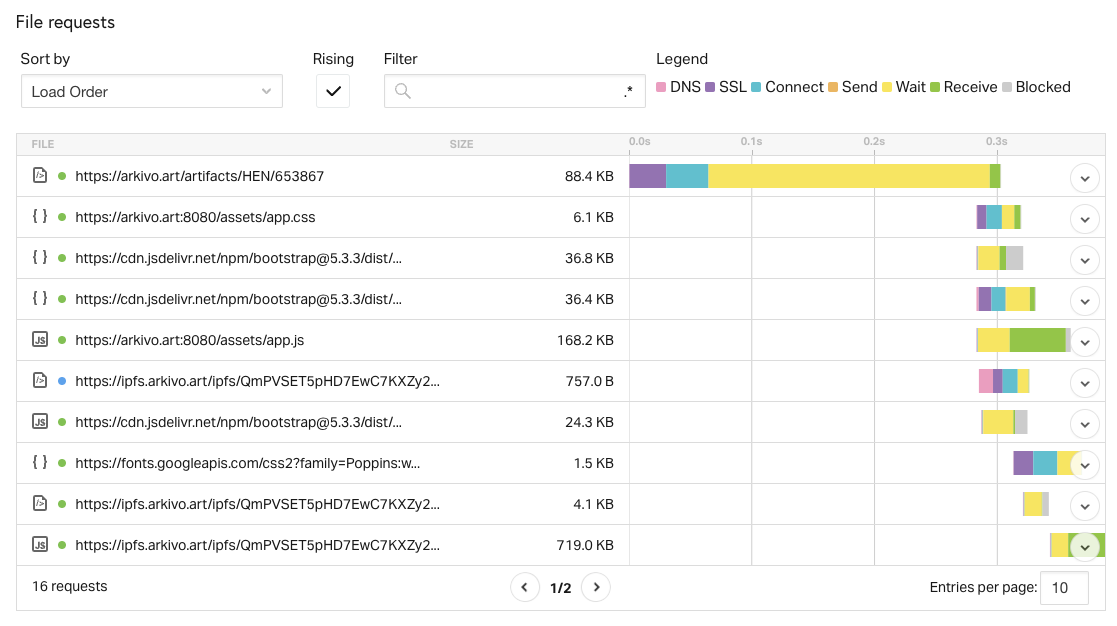
\includegraphics[width=\linewidth]{artifact-04-latency.png}
    \caption[Performance Metric: Artifact Detail Page (Loading Timeline)]{Performance Metric: Artifact Detail Page (Loading Timeline)}
    \label{fig:artifact-04-latency.png}
\end{figure}


\subsection{Web Performance Analysis}

The overall performance in terms of latency is good, although there is room for improvement. The initial page load still spends a significant amount of time in the \texttt{wait} stage, expire headers are needed, and gzip compression should also be added. Having said that, the assets loaded from the IPFS node performed better than expected.


\section{IPFS Pinning Verification}

One important outcome from developing and launching this artifact, was that it would contribute to the storage and availability of the assets from the artworks which it catalogues, by pinning their CIDs on the IPFS network. To verify that this is the case, one can use online tools which test and report whether a node does indeed do this, such as the IPFS Check tool by Fleek\footnotemark[2].

\footnotetext[2]{https://ipfs-check.on.fleek.co/}

Before doing this we need to gather some information, namely our IPFS node PeerID, and the CID of an artwork's asset that we want to test.

For the IPFS node PeerID, we need to gain shell access to the docker container:

\texttt{docker exec -it arkivo\_ipfs /bin/sh}

And then run the command:

\texttt{ipfs id}

This returns a listing as follows:

\begin{lstlisting}[language=, caption={IPFS ID Listing}, label={lst:ipfs-id}] 
{
	"ID": "12D3KooWLgNwdHQspFbSSTPSGzarCLL9iQZ4byGfaTpMNfHqBxsA",
	"PublicKey": "CAESIKFkyOEovylxWF8BqSpzIi/8CgexN5oNumjWEHg8OKSp",
	"Addresses": [
		"/ip4/127.0.0.1/tcp/4001/p2p/12D3KooWLgNwdHQspFbSSTPSGzarCLL9iQZ4byGfaTpMNfHqBxsA",
		"/ip4/127.0.0.1/udp/4001/quic-v1/p2p/12D3KooWLgNwdHQspFbSSTPSGzarCLL9iQZ4byGfaTpMNfHqBxsA",
		"/ip4/127.0.0.1/udp/4001/quic-v1/webtransport/certhash/uEiAlIZyEYPy9E79U7avKgVdYjhygiz4Z-Oxf8UqEIGQ-BA/certhash/uEiAfDpKQb46669VLVqNw__1QB27Bibr2BGU3QEnZQ4XiBQ/p2p/12D3KooWLgNwdHQspFbSSTPSGzarCLL9iQZ4byGfaTpMNfHqBxsA",
		"/ip4/167.235.68.63/tcp/4001/p2p/12D3KooWLgNwdHQspFbSSTPSGzarCLL9iQZ4byGfaTpMNfHqBxsA",
		"/ip4/167.235.68.63/udp/4001/quic-v1/p2p/12D3KooWLgNwdHQspFbSSTPSGzarCLL9iQZ4byGfaTpMNfHqBxsA",
		"/ip4/167.235.68.63/udp/4001/quic-v1/webtransport/certhash/uEiAlIZyEYPy9E79U7avKgVdYjhygiz4Z-Oxf8UqEIGQ-BA/certhash/uEiAfDpKQb46669VLVqNw__1QB27Bibr2BGU3QEnZQ4XiBQ/p2p/12D3KooWLgNwdHQspFbSSTPSGzarCLL9iQZ4byGfaTpMNfHqBxsA",
		"/ip4/172.18.0.7/tcp/4001/p2p/12D3KooWLgNwdHQspFbSSTPSGzarCLL9iQZ4byGfaTpMNfHqBxsA",
		"/ip4/172.18.0.7/udp/4001/quic-v1/p2p/12D3KooWLgNwdHQspFbSSTPSGzarCLL9iQZ4byGfaTpMNfHqBxsA",
		"/ip4/172.18.0.7/udp/4001/quic-v1/webtransport/certhash/uEiAlIZyEYPy9E79U7avKgVdYjhygiz4Z-Oxf8UqEIGQ-BA/certhash/uEiAfDpKQb46669VLVqNw__1QB27Bibr2BGU3QEnZQ4XiBQ/p2p/12D3KooWLgNwdHQspFbSSTPSGzarCLL9iQZ4byGfaTpMNfHqBxsA"
	],
	"AgentVersion": "kubo/0.29.0/3f0947b/docker",
	"Protocols": [
		"/ipfs/bitswap",
		"/ipfs/bitswap/1.0.0",
		"/ipfs/bitswap/1.1.0",
		"/ipfs/bitswap/1.2.0",
		"/ipfs/id/1.0.0",
		"/ipfs/id/push/1.0.0",
		"/ipfs/kad/1.0.0",
		"/ipfs/lan/kad/1.0.0",
		"/ipfs/ping/1.0.0",
		"/libp2p/autonat/1.0.0",
		"/libp2p/circuit/relay/0.2.0/hop",
		"/libp2p/circuit/relay/0.2.0/stop",
		"/libp2p/dcutr",
		"/x/"
	]
}
\end{lstlisting}

Our IPFS node ID, which was automatically generated the first time we started the node, appears in line 2:
\begin{center}
\texttt{12D3KooWLgNwdHQspFbSSTPSGzarCLL9iQZ4byGfaTpMNfHqBxsA}
\end{center}
For a CID to test with, we can access an artwork on the system, such as\\ \texttt{https://arkivo.art/artifacts/HEN/8333}, expand the Artifact URIs section, and click the Artifact URI, which opens the artifact's URI on a new window.

\begin{figure}[H]
    \centering
    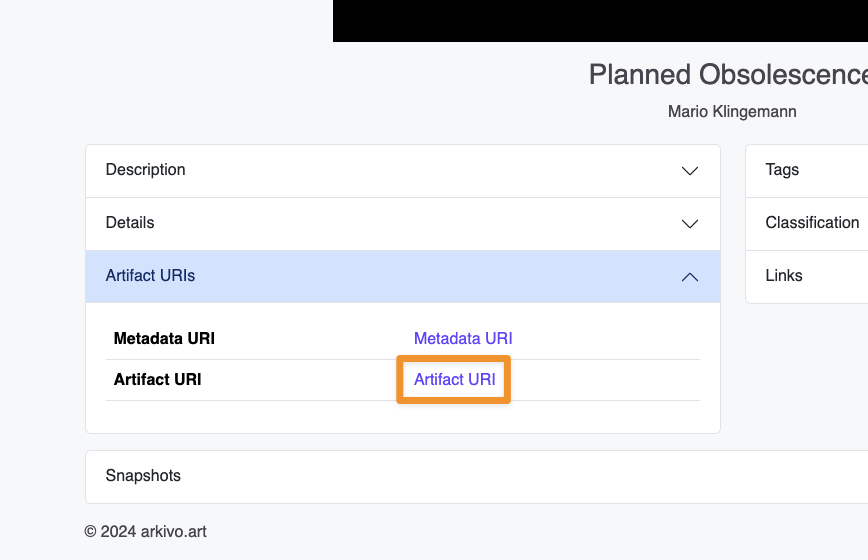
\includegraphics[width=0.5\linewidth]{how-to-find-cid1.png}
    \caption[Finding Artwork IPFS CID (part 1)]{Finding Artwork IPFS CID (part 1)}
    \label{fig:find-cid-1}
\end{figure}

The actual IPFS CID appears on the URL, between \texttt{ipfs/} and \texttt{?creator}.

\begin{figure}[H]
    \centering
    
\includegraphics[width=\linewidth]{how-to-find-cid2.png}
    \caption[Finding Artwork IPFS CID (part 2)]{Finding Artwork IPFS CID (part 2)}
    \label{fig:find-cid-1}
\end{figure}

In this example, the CID is:
\begin{center}
\texttt{QmaBAtgp6CKJwW6R4xKpNdcmjuzF132erhKExqo4wh6FCV}
\end{center}

With the \texttt{Peer ID} and the artwork's artifact CID, we can access the Fleek IPFS Check tool, and start the check. Making sure to prefix our Peer ID with \texttt{/p2p/}:

\begin{figure}[H]
    \centering
    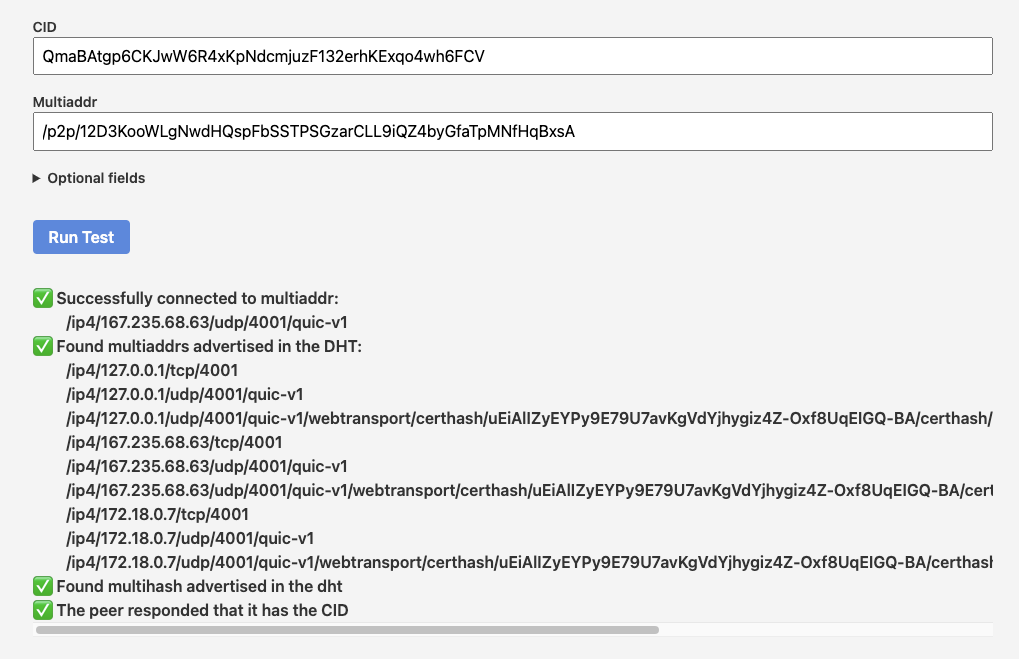
\includegraphics[width=\linewidth]{fleek-ipfs-check.png}
    \caption[Testing IPFS]{Testing IPFS}
    \label{fig:fleek-test}
\end{figure}

As can be verified in \autoref{fig:fleek-test} our node is accessible on the IPFS network, reports that it has the CID, and is also advertising its availability on the networks DHT, making it easier for other nodes to find it.

An additional check we can make is from an independent IPFS node. For example, using the IPFS node in the development server which is located in Macau, we can run a command to find IPFS nodes which are seeding a CID:

\begin{lstlisting}[language=, caption={Verification of CID availability from external node}, label={lst:ipfs-verify-macau}] 
dan@ipfs:~$ ipfs routing findprovs QmaBAtgp6CKJwW6R4xKpNdcmjuzF132erhKExqo4wh6FCV
12D3KooWAJJJwXsB5b68cbq69KpXiKqQAgTKssg76heHkg6mo2qB
12D3KooWLgNwdHQspFbSSTPSGzarCLL9iQZ4byGfaTpMNfHqBxsA
12D3KooWEHx9v2SGvFewuatTvzzGxQC1PQZPRer2ys8fYipiM1zi
12D3KooWNTSFywHjGbmGN1aEqJNp54pDKaiwqpthRrvFZETo37pW
12D3KooWNTSFywHjGbmGN1aEqJNp54pDKaiwqpthRrvFZETo37pW
12D3KooWJ8YAF6DiRxrzcxoeUVjSANYxyxU55ruFgNvQB4EHibpG
12D3KooWHEzPJNmo4shWendFFrxDNttYf8DW4eLC7M2JzuXHC1hE
12D3KooWGtYkBAaqJMJEmywMxaCiNP7LCEFUAFiLEBASe232c2VH
\end{lstlisting}

As can be seen in \autoref{lst:ipfs-verify-macau}, line 3 shows \texttt{ARKIVO}'s IPFS node. It should be noted that seeding peers are not all necessarily pinning the CID. It is simply an indication that those peers currently have a copy of the CID and are making it available to the network, but for some it could be a temporary cache and the CID could be garbage collected by those nodes at any point.

Something else worth noting is that sometimes, even when pinning content, the results from the IPFS check tool may return a failed check relating to multiash missing from the DHT, see \autoref{fig:fleek-test2}

\begin{figure}[H]
    \centering
    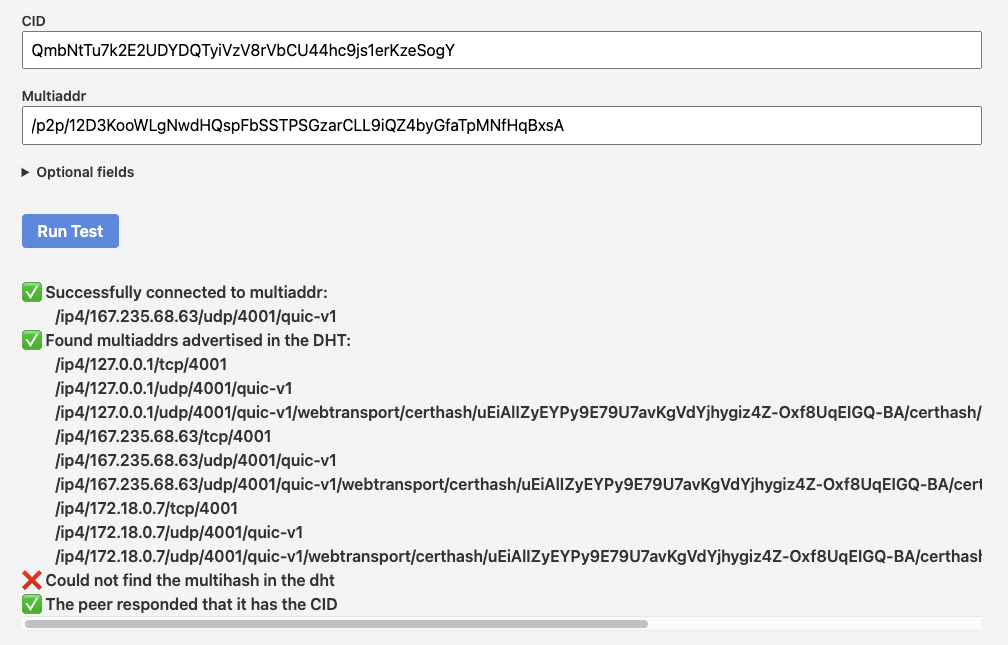
\includegraphics[width=\linewidth]{fleek-ipfs-check2.png}
    \caption[Testing IPFS (No DHT)]{Testing IPFS (No DHT)}
    \label{fig:fleek-test2}
\end{figure}

This is normal, and it is due to the fact that, by default, IPFS nodes only advertise their content every 22h \cite{KuboConfigFile2024}, and it may expire from the DHT. Normally this is not a problem, since other nodes, even those not pinning the CIDs, will likely be making them available to the network. There are tradeoffs for increasing the frequency of these provisioning messages, and normally it is a matter of hardware resources. For now we will keep the default value of 22h.


\subsection{Exhaustive IPFS Pin List Verification}

The above checks provide a very basic verification that the system is pinning content, but checking a single CID or even a handful of CIDs manually hardly constitutes a systematic evaluation of the artifact.
Therefore another method was employed, which does an exhaustive check, of every CID stored in the system's database.
The process is as follows:

\begin{enumerate}
    \item export every unique CID from the artifacts stored in the postgres database
    \item export every CID pinned by the ipfs node
    \item cross check the two data sets to find any discrepancies, such as CIDs present in one dataset but missing from the other
\end{enumerate}

Step 1, involves running the following SQL query:

\begin{lstlisting}[language=SQL, caption={SQL to export all IPFS CIDs store in DB}, label={lst:db-export-cids}] 
SELECT DISTINCT cid AS unique_cid_count
FROM (
    SELECT metadata_uri AS cid FROM artifacts
    UNION ALL
    SELECT artifact_uri AS cid FROM artifacts
    UNION ALL
    SELECT display_uri AS cid FROM artifacts
    UNION ALL
    SELECT thumbnail_uri AS cid FROM artifacts
) AS combined_cids;
\end{lstlisting}

The database exported dataset contained 47,493 records and was saved as \texttt{arkivo-db-cids.txt}. A partial listing of the file is as follows:

\begin{lstlisting}[language=, caption={Exported CIDs from postgres}, label={lst:db-export-cids-list}] 
ipfs://QmSbeMcatTg86Yjdva2RW7cQDSZtZWGpCbTMMaYNv44kuA
ipfs://QmV6G8cwEbQ1AGeQjCNDNj1kRZq4UBmmRsZi9yRr594vSh
ipfs://QmThtdTz2LD1u8uoP1zV9qtrfShcm1WSBVXHNfLTLZwHPD
ipfs://QmZuBNwDxegm6RFsU7KRxxkqy6G1y2oHiotnZqFPnMFUQx
ipfs://QmRuTHQAC3naGCxxPTCTrnrb1oXEbANhNwUwyUsaCwbhfB
...
\end{lstlisting}

Step 2, requires that we export a similar dataset from the IPFS node:

\begin{lstlisting}[language=, caption={IPFS command to export pinned CIDs}, label={lst:ipfs-export-cids}] 
ipfs pin ls --type=recursive > ipfs-node-pins.txt
\end{lstlisting}

The ipfs node exported dataset contained 46,942 records and was saved as \texttt{arkivo-db-cids.txt}. A partial listing of the file is as follows:

\begin{lstlisting}[language=, caption={Exported CIDs from IPFS node}, label={lst:ipfs-export-cids-list}] 
QmRQYgQGFjNJBudPnVEwA3jzBKaDWna943DCdCamdphdJU recursive
QmSZ2ieYnJjK9PQPrjM5Pe8ieaDfDJZJ58LuV4ijmJtayT recursive
QmUYa7jmBaWoGWAT4SdUA1R2kA7kZF4mKzMXhFYN356t2A recursive
QmWFjEUgYu6SrzSX3hJ64GHVpfNNcvWcgS9EK9hqzt2tmU recursive
QmauH5zh1UZjWoFKxQ33MW8YuepvUnUsUqzqoB3Scy6tvq recursive
...
\end{lstlisting}

There is a discrepancy of 47,493 - 46,942 = 551 records which needs to be investigated.

To perform a full cross-check between the two datasets a python program\footnotemark[3] was written that automates this process. The program ingests both files, compares them, and outputs 3 files:

\footnotetext[3]{https://github.com/seda-studio/arkivo/blob/main/utils/ipfs-pin-verification/compare-tool.py}

\begin{enumerate}
    \item \texttt{output-arkivo-cids-ok.txt} - all CIDs which are present in both datasets. These are the CIDs which are properly pinned.
    \item \texttt{output-arkivo-cids-unpinned.txt} - all CIDs present in the database file, but not pinned by the IPFS node. Any records here would be of concern.
    \item \texttt{output-ipfs-node-unknown.txt} - all CIDS pinned by the IPFS node but not in the database file. Any records here would be odd, and deserved investigation.
\end{enumerate}

After running the python script the results were as follows:


\begin{table}[h]
\footnotesize
\centering
\begin{tabular}{|l|r|}
\hline
\textbf{File} & \textbf{Total CIDs} \\ \hline
output-arkivo-cids-ok.txt                 & 46,924                         \\ \hline
output-arkivo-cids-unpinned.txt             & 569                         \\ \hline
output-ipfs-node-unknown.txt       & 18               \\ \hline
\end{tabular}
\caption{IPFS CID Pinning Cross Check Results}
\label{table:cross-check-results}
\end{table}

\subsubsection{Analysis of Unpinned CIDs}

A preliminary visual examination of \texttt{output-arkivo-cids-unpinned.txt} reveals a vast majority of unconventionally formatted entries, or even entries which are not CIDs at all. These correspond to OBJKTs which were not minted via the HEN or Teia UIs, but rather used custom minters or were just minted manually by interacting directly with the HEN smart contract, which anyone can do as the smart contract does not restrict who can interact with it.

\begin{lstlisting}[language=, caption={Unconventional Format CIDs}, label={lst:bad cids}] 
...
QmameE36rwswxEQCf6UV53kqsopD3Tprtv6km9rG1UPzHy?seed=tengil
QmameE36rwswxEQCf6UV53kqsopD3Tprtv6km9rG1UPzHy?seed=8bit
QmPVSET5pHD7EwC7KXZy2Bzah9G8UusnzcbQ7ZdcHaGi1T?seed=7az2!346fdsg4?
QmameE36rwswxEQCf6UV53kqsopD3Tprtv6km9rG1UPzHy?seed=bolitaeslaperritamasguapadeluniverso
QmameE36rwswxEQCf6UV53kqsopD3Tprtv6km9rG1UPzHy?seed=amour%20amour
QmameE36rwswxEQCf6UV53kqsopD3Tprtv6km9rG1UPzHy?seed=purespider
javascript:alert('hi');
QmameE36rwswxEQCf6UV53kqsopD3Tprtv6km9rG1UPzHy?seed=NFTs%20are%20dead
QmameE36rwswxEQCf6UV53kqsopD3Tprtv6km9rG1UPzHy?seed=Fort%20Gallery%20NfT
QmameE36rwswxEQCf6UV53kqsopD3Tprtv6km9rG1UPzHy?seed=noisynft
QmameE36rwswxEQCf6UV53kqsopD3Tprtv6km9rG1UPzHy?seed=TEZOS
...
\end{lstlisting}

One type of record consists of CIDs followed by a URL query, such `?seed=`. These are custom generative artworks which take a URL parameter as seed. The artist sets up their own website where collectors were able to input their own text as a seed to the artwork, visualise the result, and then collect that iteration as a permanently minted HEN OBJKT.

After manual analysis of the file, 4 instances of this kind of CID were found:


\begin{table}[h]
\footnotesize
\centering
\begin{tabular}{|l|r|}
\hline
\textbf{CID} & \textbf{Total records} \\ \hline
QmameE36rwswxEQCf6UV53kqsopD3Tprtv6km9rG1UPzHy	                & 430                         \\ \hline
QmPVSET5pHD7EwC7KXZy2Bzah9G8UusnzcbQ7ZdcHaGi1T	            & 62                         \\ \hline
QmWNkc1ZqEVmFxG7JDLjY4jJefkyhdwxAUegimnxFi4qSr       & 54               \\ \hline
QmVZ59sqM2QVbSXJcb8c4P9Abu35Tq3smfrFJi5VMwA3vo      & 6               \\ \hline
\textbf{Total}      &       552         \\ \hline
\end{tabular}
\caption{Custom Generative Art CIDs}
\label{table:custom-generative-cids}
\end{table}

These 4 CIDs are all from the same artist account\footnotemark[4], which belongs to generative artist @shig\_nft\footnotemark[5] , who created a series of these projects, under the name ``Procedural Symbols''. A couple of samples of the artwork are included here:

\footnotetext[4]{https://teia.art/art-o-matic}
\footnotetext[5]{https://x.com/shig\_nft}


\begin{figure}[H]
  \centering
  \begin{subfigure}[b]{0.45\textwidth}
    \centering
    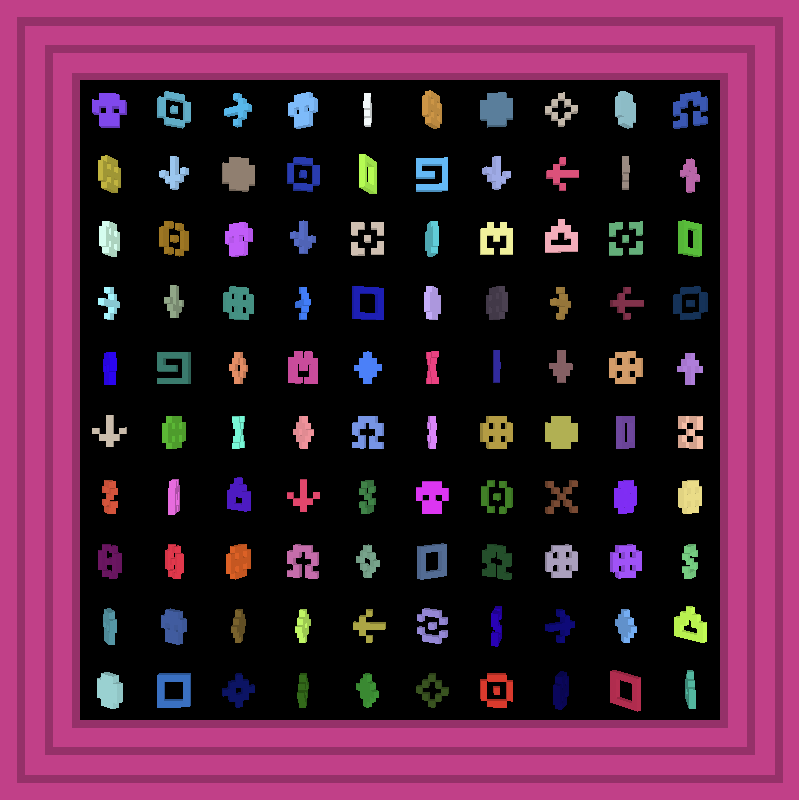
\includegraphics[width=\textwidth]{OBJKT-230702.png}
    \caption{This belongs in a museum :: Procedural Symbols \#61/1000. Source: \\https://arkivo.art/artifacts/HEN/230702\\}
    \label{fig:image1}
  \end{subfigure}
  \hfill
  \begin{subfigure}[b]{0.45\textwidth}
    \centering
    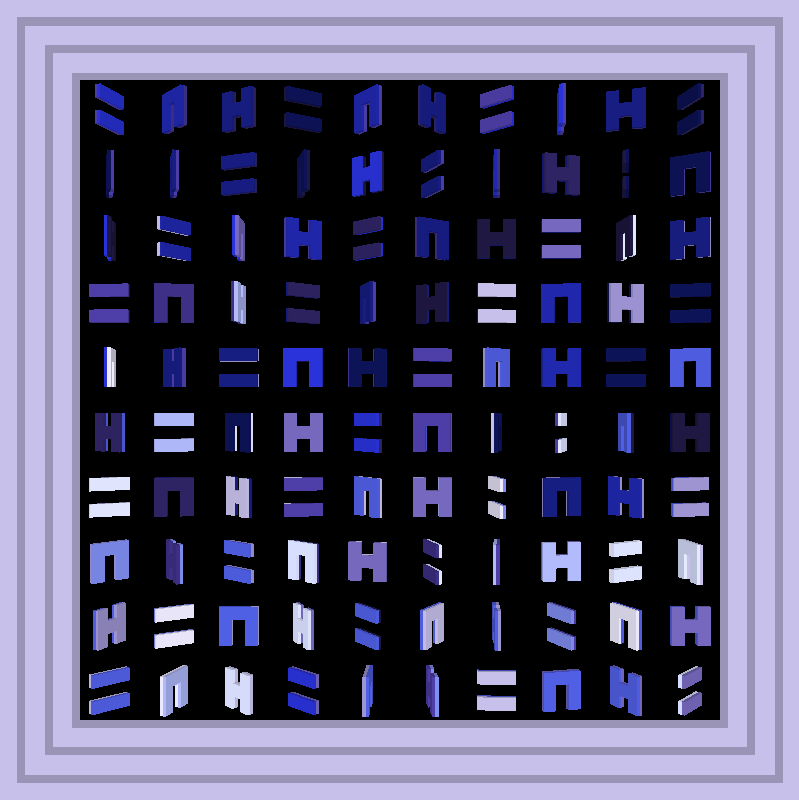
\includegraphics[width=\textwidth]{OBJKT-653867.png}
    \caption{ktorn likes blueeeeeeeeeeeeeeeeeeeee :: Procedural Symbols (H=N) \#545/1000. Source: \\https://arkivo.art/artifacts/HEN/653867}
    \label{fig:image2}
  \end{subfigure}
  \caption{Sample ``Procedural Symbols'', which add URL queries to IPFS CIDs}
  \label{fig:procedural-symbols}
\end{figure}

However the artist was also careful to mint each of the above CIDs as well formatted CID, without the URL query. This means both HEN, Teia, and now \texttt{ARKIVO} successfully pin them, and therefore those 552 records can be safely ignored as they will all work, as verified by the artworks illustrated in \autoref{fig:procedural-symbols}.

We are therefore left with 17 CIDs unaccounted for:


\begin{lstlisting}[language=, caption={17 Remaining Unconventional Format CIDs}, label={lst:17-bad-cids}] 
k51qzi5uqu5dm198e6gwnuihom8ht49z8u2qu2amjvo32380enkgfmh8riyrx9
javascript:alert('hi');
ipns/k51qzi5uqu5dhxiw7jv2i10s3o3xga5bw2wkc945zyvtpk0smrxejx632h11v4/cover.jpg
https://ipfs.io/ipns/k51qzi5uqu5dhxiw7jv2i10s3o3xga5bw2wkc945zyvtpk0smrxejx632h11v4
https://ipfs.io/ipfs/QmadbYeKWMQAiaeTmg9e7M9HQGbVjwsibPpF4rWSr5rhuk/?id=22
ipns://k51qzi5uqu5dhxiw7jv2i10s3o3xga5bw2wkc945zyvtpk0smrxejx632h11v4/cover.jpg
QmXvAQAcu1wVBCRjSoJsJczkiq18ZQ6XLjgMG7k67pBL8D?id=123
ipns://k51qzi5uqu5dhxiw7jv2i10s3o3xga5bw2wkc945zyvtpk0smrxejx632h11v4
https://ipfs.io/ipns/k51qzi5uqu5dhxiw7jv2i10s3o3xga5bw2wkc945zyvtpk0smrxejx632h11v4/cover.jpg
k51qzi5uqu5dhxiw7jv2i10s3o3xga5bw2wkc945zyvtpk0smrxejx632h11v4/cover.jpg
Qme1GBYaCfg7ZJjDBppZj4WDbvE94AD7gA5NeyLtKrvdKM?seed=SH!G%20made%20this%20%5C@/
QmU7kxXjA8mXRNEZi21joc62fCdYMgVDnErYCYr3EyH4sJ
QmfJegSaQ3SicrB6eW2XxUkYfkvvCTNkQKSAZbknmZA6zQ?seed=This is a test!
QmVQwyh9hNJVPzUmnTYFqY6bvX6PGUGxEyF1w45M9R1Brn
undefined
ipns/k51qzi5uqu5dm198e6gwnuihom8ht49z8u2qu2amjvo32380enkgfmh8riyrx9
\end{lstlisting}


After checking each one, 15 were found to be failed tests, as artists were experimenting with the possibilities. Most belong to OBJKTs which have been burned by the artists. However 2 CIDs were found to be valid and belong to existing artworks indexed by our artifact.

\begin{lstlisting}[language=, caption={17 Remaining Unconventional Format CIDs}, label={lst:17-bad-cids}] 
QmU7kxXjA8mXRNEZi21joc62fCdYMgVDnErYCYr3EyH4sJ
QmVQwyh9hNJVPzUmnTYFqY6bvX6PGUGxEyF1w45M9R1Brn 
\end{lstlisting}

Both are thumbnails, belonging to OBJKTs 767305 and 796127, respectively. It is unclear why these 2 CIDs, out of a total 46,924 CIDs, failed to get pinned. The ipfs pinning worker, similarly to the snapshot worker, will re-try an operation 3 times, as per the configuration of the redis queue. However these retries are immediate, and not delayed, so a temporary network issue, or some other problem could have affected these.

Nevertheless, one of the CLI management commands that we developed allow us to issue a pin request for any OBJKT. The syntax for the command is:\\
{
\footnotesize{\texttt{node ace artifacts:pin <blockchain> <smart-contract-address> <token-id>}}\\
}


This command will attempt a pin (or re-pin) of all CIDs associated with an OBJKT: metadata, artifact, display, and thumbnail.
\begin{lstlisting}[language=, caption={Command to Pin OBJKT}, label={lst:17-bad-cids}] 
# node ace artifacts:pin tezos KT1RJ6PbjHpwc3M5rw5s2Nbmefwbuwbdxton 767305
chain: [tezos]
contract: [KT1RJ6PbjHpwc3M5rw5s2Nbmefwbuwbdxton]
token_id: [767305]
[ info ]  Token sent for processing: 767305
#
# node ace artifacts:pin tezos KT1RJ6PbjHpwc3M5rw5s2Nbmefwbuwbdxton 796127
chain: [tezos]
contract: [KT1RJ6PbjHpwc3M5rw5s2Nbmefwbuwbdxton]
token_id: [796127]
[ info ]  Token sent for processing: 796127
\end{lstlisting}

To verify that the command worked, we tried to access the URLs from our IPFS node before and after running it.


\begin{figure}[H]
    \centering
    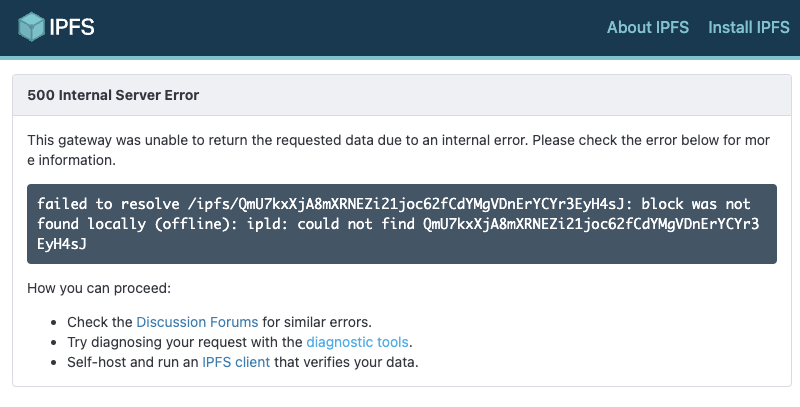
\includegraphics[width=0.75\linewidth]{before-pin.png}
    \caption[OBJKT thumbnail before pin]{OBJKT thumbnail before pin}
    \label{fig:before-pin}
\end{figure}


\begin{figure}[H]
  \centering
  \begin{subfigure}[b]{0.45\textwidth}
    \centering
    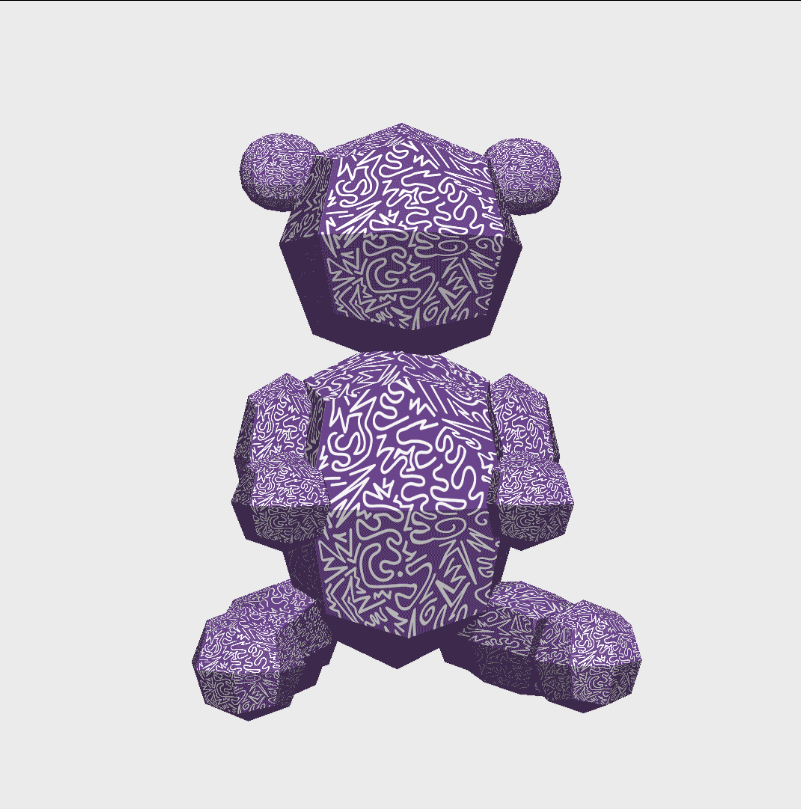
\includegraphics[width=\textwidth]{767305-thumb.png}
    \caption{``Purple Haze - Teddi'' by killjoyink. Source: \\https://arkivo.art/artifacts/HEN/767305}
    \label{fig:purple-haze}
  \end{subfigure}
  \hfill
  \begin{subfigure}[b]{0.45\textwidth}
    \centering
    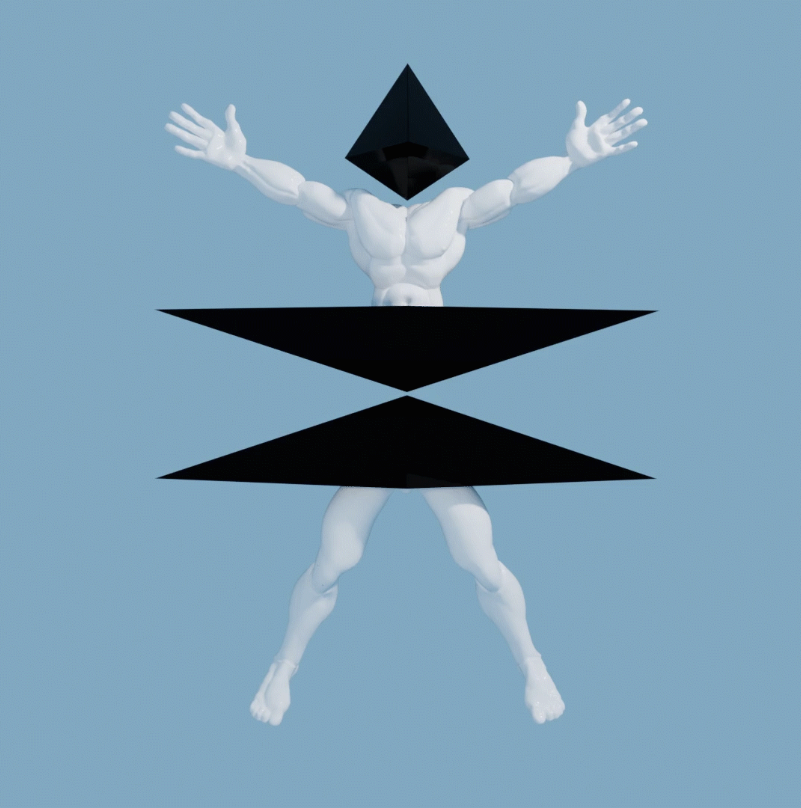
\includegraphics[width=\textwidth]{796127-thumb.png}
    \caption{``Freedom'' by Vlas Belov art. Source: \\https://arkivo.art/artifacts/HEN/796127}
    \label{fig:freedom}
  \end{subfigure}
  \caption{OBJKT thumbnails after pin retry}
  \label{fig:2-repinned-cids}
\end{figure}

With this, we can now conclude that all valid CIDs are successfully pinned by our IPFS node. However we still have 18 CIDs pinned by the IPFS node which are not in our database, therefore unaccounted for.


\subsubsection{Analysis of Unknown CIDs}

The list of 18 unknown CIDs is as follows:

\begin{lstlisting}[language=, caption={Command to Pin OBJKT}, label={lst:18-unknown-cids}] 
QmVi33nTqwUZbL64d7Ab9EPPW4npmQRxMhE1E8VQnQZsHf
QmaxptTRV7we3QubVsiNcpSf74zmCrsKrXYS1wH6NfjHDm
QmYBWDdBpQwP1QgPZo94Mx8VM6XNr2xRmpVhAcLrHhZNhd
QmU9eBL6T7zAGV48o462LDvB4YPNnYjpmgQDQaB7PTboNP
QmdcamM7GogJxh3uBQkoGkw7CpJzghbVubFknvTw9tNPpm
QmacVsizqR49aqeKaxWCVBuD77mbKh9xf2CRnVJ6aPkRQq
Qmd5mT8GYEeDp2zG5jqEndZKoqn882FMzcbFmYdhxzrubz
QmZRUBYuDfsT1oWzD91ZdHbnrBsaSY78awYoB9ihAfn3df
Qmd8w32fPqa1niDQpQqooxznhB5qjsFdmw713pcDcaV6VW
QmTHGKahi8bG4W6MV4bsvjSpgr6DThiWP9LbhT1extuwpU
QmPgLV9BVygyPy3x3C3qNWGWJoJZtDD5P4JAVXq6g7siG9
QmTCaF4prs5ndNVsBoCsHGHBRYyLLKQeryTyA6hDtMTk1R
Qme1GBYaCfg7ZJjDBppZj4WDbvE94AD7gA5NeyLtKrvdKM
QmcSfymXa4rgip9QdqmP8xFNERBmLdWZxd3vGkN7QxMR75
QmRzvn7672UYPniAvz4ofh9dmDNF2NvjEeyBtBEvbcuQ29
QmYuApfJaKy8tcMCrjgjQ8nGMdqrq75kQ5qA5aSikCD96F
QmVp8W3xQCCFU4PHrUQgyb4yfFeR1SL3gM2xtvS6sdEiK8
QmUNLLsPACCz1vLxQVkXqqLX5R1X345qqfHbsf67hvA3Nn
\end{lstlisting}

Two of the CIDs were done manually as a means to test the IPFS node, so are accounted for. However the 16 remaining ones are unknown, and the vast majority seem to be trailers for a Chinese TV soap opera.
The most plausible theory is that, during the deployment of the artifact in production, a few hours elapsed in which the firewall was not yet in place, and remote nodes were able to access our node's private API port (5001) and remotely requested the pinning of those CIDs.

Since we already have the firewall in place now, it is just a matter of cleaning those CIDs from our node, which we did with the command: \texttt{ipfs pin rm <CID>}, followed by a \texttt{ipfs repo gc} to garbage collect any remains of CIDs which should not be there.

Additionally, we enabled the option \texttt{NoFetch = true} on the IPFS node configuration, which ensures our node only serves content which is explicitly pinned, and will not attempt to fetch any other CIDs requested via the public gateway. Only requests from our application, via the (now private) API port will pin new content to our node.

This was an invaluable, as well as slightly comical, lesson and reminder on how to deploy IPFS nodes, or any other application for that matter: have the firewall in place \emph{before} deployment!

\subsection{Verifying IPFS Data Integrity}

Verifying that all CIDs are pinned is only half of the work. We also need to check the data integrity of all pinned content on the node. To achieve that, IPFS offers a command which exhaustively checks the data integrity of every pinned CID: \texttt{ipfs pin verify}. This command can take some time to complete, with over 46000 CIDs to verify, for that reason the command was prefixed by \texttt{time} to determine how long it takes to execute.

\begin{lstlisting}[language=, caption={Internal IPFS pin verification}, label={lst:ipfs-pin-verification}] 
/ # time ipfs pin verify
real	5m 30.82s
user	0m 0.07s
sys	  0m 0.05s
\end{lstlisting}

As can be seen in \autoref{lst:ipfs-pin-verification}, it ran in 5m30s and returned no errors, therefore our storage's integrity is verified.


\section{Snapshot Verification}

Verifying the validity of the snapshots is significantly more difficult, because many things could go wrong unnoticed, for example a screenshot could fail to capture the rendering of the artwork.

\begin{enumerate}
    \item Verify that every artifact has one, and only one, snapshot recorded in the database;
    \item Perform a systematic visual check of the screenshots
    \item Perform a manual verification that the classification of artworks as networked is correct
\end{enumerate}

\subsection{Snapshot Record Integrity Verification}

Here we want to run a SQL query that verifies that each artifact in the database has exactly one snapshot. 

The first query we run checks if any artifacts do not have a snapshot:

\begin{lstlisting}[language=SQL, caption={SQL - Check Missing Snapshots}, label={lst:sql-missing-snapshots}] 
SELECT COUNT(id)
FROM artifacts
WHERE id NOT IN (
    SELECT DISTINCT artifact_id
    FROM snapshots
);
\end{lstlisting}

And unfortunately we have a total of \texttt{174}. Similarly to the IPFS pinning worker, our snapshoting worker retries 3 times before giving up, so something wrong must be happening with these artifacts.

After exporting the list of token\_ids affected,  another batch of snapshots was started, just for those artifacts. It became clear that something is indeed preventing these artifacts from getting snapshotted, with Playwright reporting several timeout errors. A visual inspection of a selection of the artifacts proved that it was loading on the web UI, so the IFPS asset was present in the system. One observation was that all these artifacts were quite \emph{heavy} in terms of CPU load, making the fan on the computer spin up. This could be an indication of the problem. After the batch of snapshots completed, the SQL query was retried and this time the number went down to \texttt{164}. This means 10 artifacts out of 174, succeeded in getting snapshotted this time around.

Since we are indexing and hosting 21,390 artifacts, 164 represents only 0.766\% of the total, so it was decided that the snapshots for these artifacts would have to be revisited at a later stage.

The reverse query was then used to find artifacts that may have more than one snapshot.


\begin{lstlisting}[language=SQL, caption={SQL - Check Duplicate Snapshots}, label={lst:sql-missing-snapshots}] 
SELECT COUNT(*)
FROM (
    SELECT artifact_id, COUNT(*) AS snapshot_count
    FROM snapshots
    GROUP BY artifact_id
    HAVING COUNT(*) >= 2
) AS subquery;
\end{lstlisting}

This returned a surprising count of \texttt{4345}. A quick follow-up query revealed 13 artifacts with 3 snapshots each, followed by a long tail of artifacts with 2 snapshots. This represents nearly 20\% of all artifacts having more than one snapshot. Since only one batch of snapshots was run, this could mean that there is an issue on the snapshot retry logic. A note was taken of this for future troubleshooting, and the duplicate snapshots were removed:

\begin{lstlisting}[language=SQL, caption={SQL - Deleting Duplicate Snapshots}, label={lst:sql-missing-snapshots}] 
DELETE FROM snapshots
WHERE id NOT IN (
    SELECT id FROM (
        SELECT id,
               ROW_NUMBER() OVER (PARTITION BY artifact_id ORDER BY created_at DESC) AS rn
        FROM snapshots
    ) AS ranked
    WHERE rn = 1
);
\end{lstlisting}

This concluded the basic snapshot record integrity check. Now we need to look into the actual content of the snapshots.

\subsection{Snapshot Visual Verification}

At a first glance the snapshot seems to have identified the external network call, and ignored the internal ones. It also captured the screenshot well.
The full snapshot download worked as well. To verify that the network call was well identified it was run with the browser's developer tools open. 

\begin{figure}[h]
    \centering
    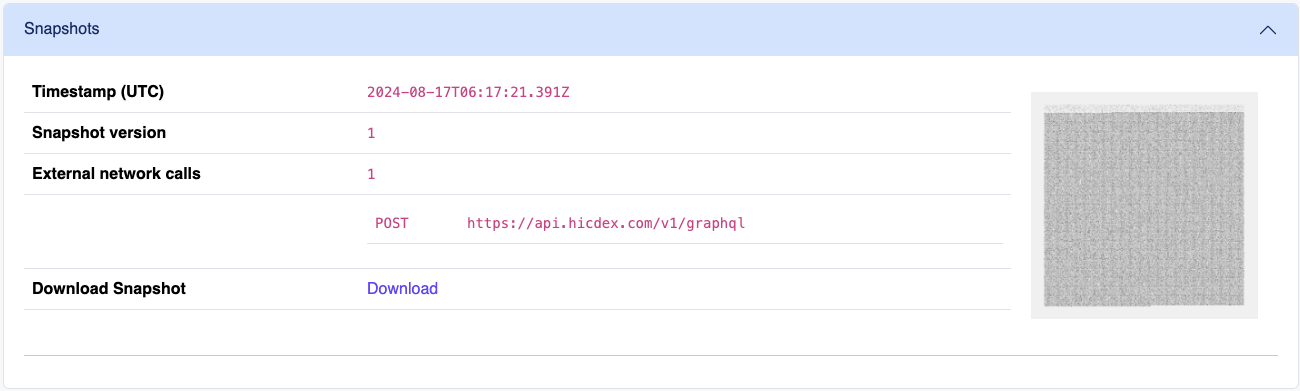
\includegraphics[width=\linewidth]{snapshot-sample.png}
    \caption[Sample Snapshot]{Sample Snapshot}
    \label{fig:sample-snapshot}
\end{figure}

Additionally, the automatic classification was checked for correctness. It also passed, see \autoref{ig:sample-classfication}.

\begin{figure}[h]
    \centering
    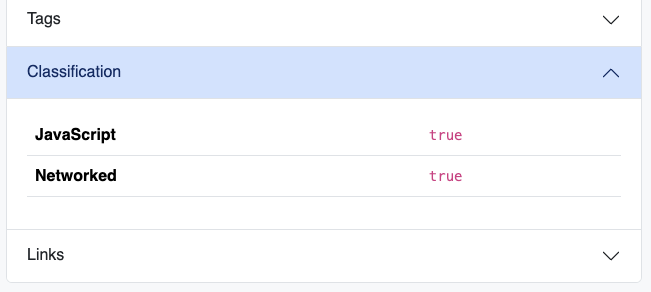
\includegraphics[width=0.5\linewidth]{sample-classification.png}
    \caption[Sample Classification]{Sample Classification}
    \label{fig:sample-classfication}
\end{figure}


After this initial check a systematic verification took place. For every 50 pages of results, the first artifact on the page was checked following the same procedure as above. A total of 36 artifacts were manually verified and all passed the test.

At this stage we were ready to involve stakeholders in the evaluation of the artifact.


\subsection{Stakeholder Feedback}

Several stakeholders were contacted, via twitter and discord, however due to lack of time, only 

The 'Networked Only' checkbox caused some confusion, as one user assumed it was a filter which should instantly be reflected on the results as one checks or unchecks it. Although not originally intended as an auto-updating filter (actual filters were not implemented) the behaviour of the checkbox was altered, by adding an \texttt{onchange} event which submits the form every time it is checked or unchecked. This results in an experience that is more aligned with the user's expectations, and is a reasonable compromise until a proper filtering system is put in place.




\section{Data Analysis}

boilerplate text, boilerplate text, boilerplate text, boilerplate text, boilerplate text, boilerplate text, boilerplate text, boilerplate text, boilerplate text, boilerplate text.


\section{Restoration Case Studies}

\todo


\section{Archiving ARKIVO}

As discussed in \todo, Teia's current UI prevents the WayBackMachine from successfully capturing the OBJKTs displayed on each page. By employing a simpler Web UI, \texttt{ARKIVO} allows such archiving. As an example we requested the capture of ``Generative Abstract Series 012'' by Yazid via the \texttt{ARKIVO} page, and the capture completed successfully, see \autoref{fig:awayback-arkivo}. This gives artworks catalogued by our system a chance of gaining yet another archival copy, and these copies could even outlast \texttt{ARKIVO} itself.


\begin{figure}[h]
    \centering
    \captionsetup{justification=centering}
    \begingroup
    \setlength{\fboxsep}{0pt} % No padding between box and content
    \setlength{\fboxrule}{1pt} % Thickness of the border
    \fcolorbox{gray}{white}{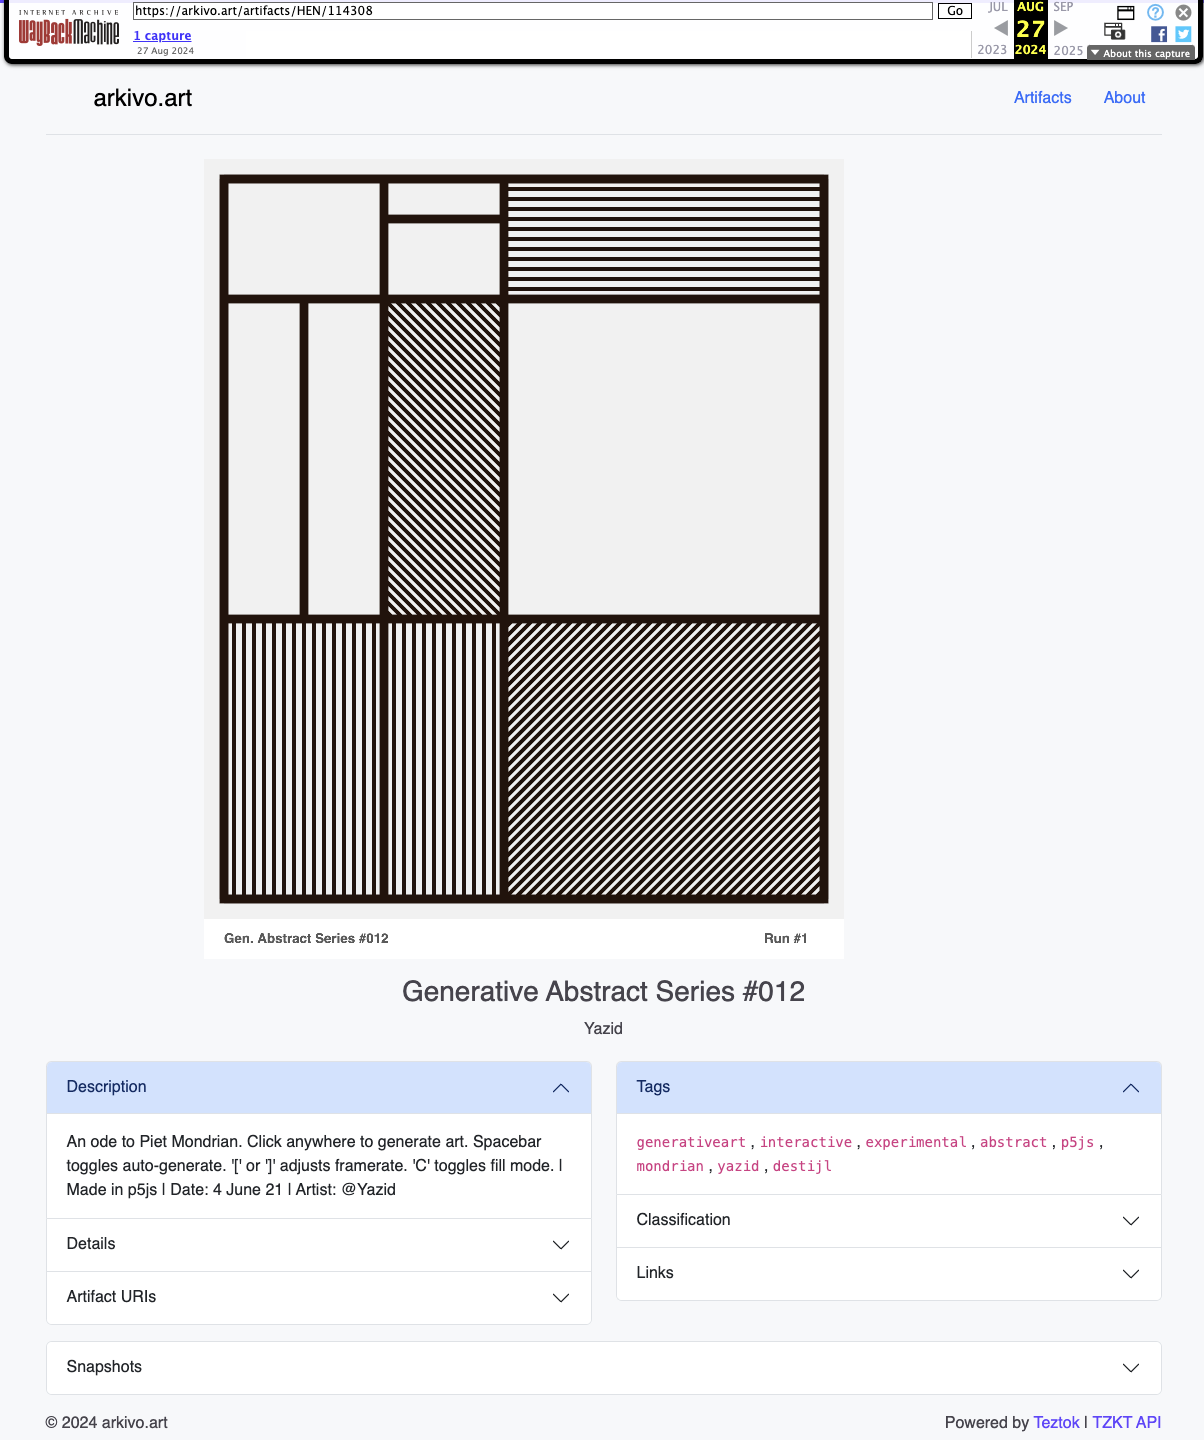
\includegraphics[width=0.75\linewidth]{wayback-and-arkivo.png}}
    \endgroup
    \caption[WayBackMachine snapshots Arkivo]{Generative Abstract Series 012 by Yazid, \\ a snapshot of Arkivo by WayBackMachine}
    \label{fig:awayback-arkivo}
\end{figure}


\section{Discussion}


boilerplate text, boilerplate text, boilerplate text, boilerplate text, boilerplate text, boilerplate text, boilerplate text, boilerplate text, boilerplate text, boilerplate text.


\subsection{Capturing Interactive Artworks}
\label{subsec:capture-interactive}

One of the challenges of automating the aesthetic capture of user-interactive artworks is determining the ways in which they can be interacted with. As discussed in \autoref{sec:interactivity}, interactions can take many forms. However a manual non-exhaustive sampling of OBJKTs indexed by \texttt{ARKIVO} suggests that mouse and keyboard interactions are the most common forms of interaction in this dataset. Tools like PlayWright can simulate mouse and keyboard input during the snapshotting process, so in theory it should be possible to capture this kind of interaction. However the biggest challenge in achieving automatic interaction without any prior knowledge of the artwork is determining where in the screen to click or which keys to press. Also depending on the nature of the artwork, the interactions could be quite complex.

However a very basic experiment was attempted, using ChatGPT, to determine if a piece is interactive, and if so, where in the screen to click. As an example, the ``Jumpy Dot'' artwork by mrdoob was used.

After uploading the screenshot, the following prompts, designed to be generic and applicable to all artworks indexed by \texttt{ARKIVO}, were used:

\begin{enumerate}
	\item examine this image, and tell me if you think this represents an interactive interface
	\item if I were to click on the image to interact with it, give me approximate x,y coordinates where I should click
\end{enumerate}


The full ChatGPT chat with prompts and responses can be found in Appendix 3, page \pageref{chap:chatgpt-mouse}.

ChatGPT successfully identified the 'start' button and thus correctly classified the artwork as interactive. It also provided the following \texttt{X,Y} coordinates for click it: \texttt{255, 350}

As can be seen in \autoref{fig:chat-gpt-click-guess}, the coordinate provided by ChatGPT was relatively close, but failed to hit the 'start' button.

\begin{figure}[H]
  \centering
  \begin{subfigure}[b]{0.45\textwidth}
    \centering
    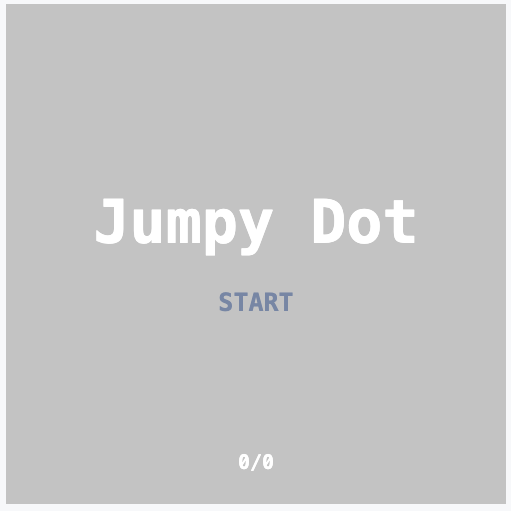
\includegraphics[width=\textwidth]{jumpydot.png}
    \caption{Input screenshot}
    \label{fig:image1}
  \end{subfigure}
  \hfill
  \begin{subfigure}[b]{0.45\textwidth}
    \centering
    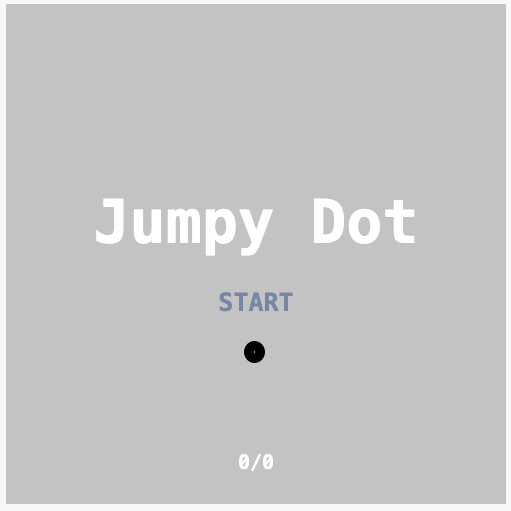
\includegraphics[width=\textwidth]{jumpydot-click.png}
    \caption{ChatGPT coordinate guess}
    \label{fig:image2}
  \end{subfigure}
  \caption{ChatGPT estimated interaction coordinate}
  \label{fig:chat-gpt-click-guess}
\end{figure}

It should be noted that this artwork, due to the simplicity its the interface, and the explicit nature of the 'start' button, constitutes one of the easiest possible tests for an LLM like ChatGPT to determine interactivity and hotspot locations for interactions. The fact that it failed to provide the correct coordinate suggests there is still a gap between the textual description of the location of the button, "close to the center horizontally [...] slightly below the center vertically" and the prediction of the coordinate.

The LLM approach to UI interaction is fairly new, but some research is starting emerge \cite{liuMakeLLMTesting2024}, and more is expected to follow.

Alternative strategies for interacting with the artwork can also be experimented with. For example, the Android development ecosystem has a tool, UI/Application Exerciser Monkey, which generates pseudo-random streams of user events such as clicks, touches, or gestures for automated UI testing \cite{UIApplicationExerciser}.

\subsection{Cost of Storage}

Currently, the cost of minting an OBJKT on the HEN contract constitutes a fraction of the cost of hosting and/or pinning 2GB of data. This represents a loophole that could be exploited by malicious actors, or freeloaders, making the pinning of assets hosted by Teia unfeasible without a significant recurring investment, which impacts the economic sustainability of the project.

\subsection{Emulation}

As time passes, technology will continue to evolve. New hardware will run new operating systems, which will run new web browsers, or even totally paradigm changing \emph{content rendering applications} which may replace web browsers in the future. This means that in long term it seems inevitable that all code-base artworks created today, even those based on web standards and without any network dependencies, will require some form of hardware and/or browser emulation to render successfully. 

This inevitable evolution into emulated environments does represent an additional challenge for networked artworks, because in addition to emulating the artefact's code-base itself, the emulation environment must also simulate the network dependencies of the artwork, and this can pose a problem known to software developers as \emph{dependency hell}, where each dependency in turn depends on a number of other dependencies, leading to an ever increasing dependency tree. A solution to this problem seems unfeasible, if any of those dependencies, or their sub-dependencies, does not strictly follow the web3 architecture that makes projects easily duplicable.

For this reason, the IOC model gains an even greater importance for the longevity of code-based networked artworks, because you can more easily generate the data expected by the artwork, or in the worst-case scenario, simply repeatedly inject the last known good snapshot of data for all future renderings.

\subsection{Beyond the Canvas}

All of the artworks which this project currently aims to cater for in terms of conservation have one thing in common: their visual rendering is restricted to the boundaries of an HTML element on a web page, the canvas. Even those which intentionally choose to spread their visual expression past the boundaries of a single canvas element, are still constrained by the larger HTML DOM object or web page in which they, as web-based artworks, essentially exist. This is not unique to digital art. The great majority of paintings displayed in traditional museums are also constrained by their physical framed canvasses. Sculptures and other art installations are exceptions to this rule. However networked art reaches out into the world, and it would seem appropriate to explore a rendering medium that represents that breaking away from the canvas.


\subsection{Identifying IPFS Pinning Abuse}

Since most IPFS pinning services are paid for, there is a potential for abuse of free pinning services like Teia, and now Arkivo, by mining directory-x OBJKTs just as a way to store data on IPFS for free. The OBJKT might even render a piece of original art, but just as a facade for a much larger data payload. This would add to an archive's storage costs without contributing back in terms of donation, hurting its sustainability.


On the other hand, if the art has value, 

